\chapter{Recurrent Neural Networks}
\label{chap-rnn}

So far, we have limited our attention to domains in which each output
$y$ is assumed to have been generated as a function of an associated
input $x$, and our hypotheses have been ``pure'' functions, in which
the output depends only on the input (and the parameters we have
learned that govern the function's behavior).  In the next few
chapters, we are going to consider cases in which our models need to
go beyond functions.  In particular, behavior as a function of {\em
    time} will be an important concept:
\begin{itemize}
  \item In {\em recurrent neural networks}\index{recurrent neural
          network}, the hypothesis that we learn is not a function of a single
        input, but of the whole sequence of inputs that the predictor has
        received.
  \item In {\em reinforcement learning}\index{reinforcement learning},
        the hypothesis is either a {\em model} of a domain (such as a game)
        as a recurrent system or a {\em policy} which is a pure function,
        but whose loss is determined by the ways in which the policy
        interacts with the domain over time.
\end{itemize}

In this chapter, we introduce {\em state machines}\index{state machine}.
We start with deterministic state machines, and then consider
recurrent neural network (RNN) architectures to model their behavior.
Later, in Chapter~\ref{chap-mdps}, we will study {\em Markov decision
    processes} (MDPs) that extend to consider probabilistic (rather than
deterministic) transitions in our state machines.
RNNs and MDPs will enable description and modeling of temporally
sequential patterns of behavior that are important in many domains.


%%%%%%%%%%%%%%%%%%%%%%%%%%%%%%%%%%%%%%%%%%%%%%%%%%%%%%%%%%%%%%%%%%%%%%%%%%%%%
\section{State machines}
\label{sec-state_machines}

A {\em state machine} \note{This is such a pervasive idea that it has
been given many names in many subareas of computer science, control
theory, physics, etc., including: {\em automaton}, {\it transducer},
{\it dynamical system}, etc.}  is a description of a
process (computational, physical, economic) in terms of its potential
sequences of {\em states}.

The {\em state} of a system is defined to be all you would need to
know about the system to predict its future trajectories as well as
possible.  It could be the position and velocity of an object or the
locations of your pieces on a game board, or the current traffic
densities on a highway network.

Formally, we define a {\em state machine} as
$(\mathcal{S}, \mathcal{X}, \mathcal{Y}, s_0, f_s, f_o)$
where
\begin{itemize}
  \item $\mathcal{S}$ is a finite or infinite set of possible states;
  \item $\mathcal{X}$ is a finite  or infinite  set of possible inputs;
  \item $\mathcal{Y}$ is a finite or infinite set of possible outputs;
  \item $s_0 \in \mathcal{S}$ is the initial state of the machine;
  \item $f_s: \mathcal{S} \times \mathcal{X} \rightarrow \mathcal{S}$ is a
          {\em transition function}\index{transition function}, which takes an
        input and a previous state and produces a next state;
  \item $f_o: \mathcal{S} \rightarrow \mathcal{Y}$ is an {\em output
            function}\index{output function}, which takes a state and produces
        an output.
\end{itemize}

The basic operation of the state machine is to \note{In some cases, we
  will pick a starting state from a set or distribution.}  start with
state $s_0$, then iteratively compute for $t \geq 1$:
\begin{align}
  s_t & = f_s(s_{t - 1}, x_t) \\
  y_t & =  f_o(s_t)
\end{align}
\begin{examplebox}
  The diagram below illustrates this process.  Note that the
  ``feedback'' connection of $s_t$ back into $f_s$ has to be buffered or
  delayed by one time step----otherwise what it is computing would not
  generally be well defined.
  \begin{center}
    \tikzstyle{block} = [draw, fill=blue!20, rectangle, minimum height=3em, minimum width=3em]
    \tikzstyle{sum} = [draw, fill=blue!20, circle, node distance=1cm]
    \tikzstyle{input} = [coordinate]
    \tikzstyle{output} = [coordinate]
    \tikzstyle{pinstyle} = [pin edge={to-,thin,black}]

    % The block diagram code is probably more verbose than necessary
    \begin{tikzpicture}[auto, node distance=2cm,>=latex']
      % We start by placing the blocks
      \node [input, name=input] {};
      \node [block, right of=input, node distance=2cm] (f) {$f_s$};
      \node [block, right of=f,
        node distance=4cm] (g) {$f_o$};
      % We draw an edge between the controller and system block to 
      % calculate the coordinate u. We need it to place the measurement block. 
      \draw [->] (f) -- node[name=u] {$s_t$} (g);
      \node [output, right of=g, node distance=2cm] (output) {};
      \node [coordinate, name=measurements, below of=f, node distance=2cm] (measurements) {Measurements};

      % Once the nodes are placed, connecting them is easy. 
      \draw [draw,->] (input) -- node {$x_t$} (f);
      \draw [->] (g) -- node [name=y_t] {$y_t$}(output);
      \draw [->] (u) |- (measurements);
      \draw [->] (measurements) -| node[pos=0.99] {$-$}
      node [near end] {$s_{t - 1}$} (f);
    \end{tikzpicture}
  \end{center}
\end{examplebox}
So, given a sequence of inputs $x_1, x_2, \dots$ the machine generates a
sequence of outputs
$$ \underbrace{f_o(f_s(s_0, x_1))}_{y_1}, \underbrace{f_o(f_s(f_s(s_0, x_1), x_2
    ))}_{y_2}, \dots \;\;.$$
We sometimes say that the machine {\em  transduces} sequence  $x$ into
sequence $y$.
The output at time $t$ can have dependence on inputs from steps $1$ to
$t$.\note{There are a huge
  number of major and minor variations on the idea of a state machine.
  We'll just work with one specific one in this section and another
  one in the next, but don't worry if you see other variations out in
  the world!}

One common form is {\em finite state machines}\index{finite state
  machine}, in which $\mathcal S$, $\mathcal X$, and $\mathcal Y$ are
all finite sets.  They are often described using {\em state transition
    diagrams}\index{state transition diagram} such as the one below, in
which nodes stand for states and arcs indicate transitions.  Nodes are
labeled by which output they generate and arcs are labeled by which
input causes the transition.  \note{All computers can be described, at
  the digital level, as finite state machines.  Big, but finite!}

\begin{examplebox}
  One can verify that the state machine below reads binary strings and
  determines the parity of the number of zeros in the given string.
  Check for yourself that all input binary strings end in state $S_1$ if
  and only if they contain an even number of zeros.
  \begin{center}
    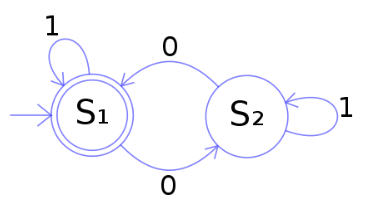
\includegraphics[scale=1.0]{figures/FSM.png}
  \end{center}
\end{examplebox}

Another common structure that is simple but powerful and used in
signal processing and control is {\em linear time-invariant (LTI)
    systems}\index{linear time-invariant systems}.  In this case, all
the quantities are real-valued vectors: $\mathcal S = \R^m$, $\mathcal
  X = \R^l$ and $\mathcal Y = \R^n$. The functions $f_s$ and $f_o$ are
linear functions of their inputs.
The transition function is described by the state matrix $A$ and the input matrix $B$;
the output function is defined by the output matrix $C$, each with compatible dimensions.
In discrete time, they can be
defined by a linear difference equation, like
\begin{align}
  s_t & = f_s(s_{t-1}, x_t) = A s_{t-1} + B x_t, \\
  y_t & = f_o(s_t) = C s_t, \;\;
\end{align}
and can be implemented using state to store relevant previous
input and output information.
We will study {\it{recurrent neural networks}} which are a lot like a
non-linear version of an LTI system.


%%%%%%%%%%%%%%%%%%%%%%%%%%%%%%%%%%%%%%%%%%%%%%%%%%%%%%%%%%%%%%%%%%%%%%%%%%%%%
\section{Recurrent neural networks}
\label{sec-rnn_model}

In Chapter~\ref{chap-neural_networks}, we studied neural networks and
how the weights of a network can be obtained by training on data, so
that the neural network will model a function that approximates the
relationship between the $(x, y)$ pairs in a supervised-learning
training set.  In Section~\ref{sec-state_machines} above, we
introduced state machines to describe sequential temporal
behavior. Here in Section~\ref{sec-rnn_model}, we explore recurrent
neural networks by defining the architecture and weight matrices in a
neural network to enable modeling of such state machines.  Then, in
Section~\ref{sec-seq2seq_rnn}, we present a loss function that may be
employed for training {\em sequence to sequence} {\sc rnn}s, and then
consider application to language translation and recognition in
Section~\ref{sec-language}.  In Section~\ref{sec-bptt}, we'll see how
to use gradient-descent methods to train the weights of an {\sc rnn}
so that it performs a {\em transduction} that matches as closely as
possible a training set of input-output {\em sequences}.

\bigskip

\begin{comment}
Recall that the basic operation of the state machine is to
start with some state $s_0$, then iteratively compute for $t \geq 1$:
\begin{align}
  s_t & = f_s(s_{t - 1}, x_t) \\
  y_t & =  f_o(s_t)
\end{align}
as illustrated in the diagram below (remembering that there needs to
be a delay on the feedback  loop):
\begin{center}
  \tikzstyle{block} = [draw, fill=blue!20, rectangle, minimum height=3em, minimum width=3em]
  \tikzstyle{sum} = [draw, fill=blue!20, circle, node distance=1cm]
  \tikzstyle{input} = [coordinate]
  \tikzstyle{output} = [coordinate]
  \tikzstyle{pinstyle} = [pin edge={to-,thin,black}]

  % The block diagram code is probably more verbose than necessary
  \begin{tikzpicture}[auto, node distance=2cm,>=latex']
    % We start by placing the blocks
    \node [input, name=input] {};
    \node [block, right of=input, node distance=2cm] (f_s) {f_s};
    \node [block, right of=f,
      node distance=4cm] (f_o) {f_o};
    % We draw an edge between the controller and system block to 
    % calculate the coordinate u. We need it to place the measurement block. 
    \draw [->] (f) -- node[name=u] {\hspace*{1cm} $s_t$} (f_o);
    \node [output, right of=f_o, node distance=2cm] (output) {};
    \node [coordinate, name=measurements, below of=f, node distance=2cm] (measurements) {Measurements};

    % Once the nodes are placed, connecting them is easy. 
    \draw [draw,->] (input) -- node {$x_t$} (f_s);
    \draw [->] (f_o) -- node [name=y_t] {$y_t$}(output);
    \draw [->] (u) |- (measurements);
    \draw [->] (measurements) -| node[pos=0.98] {$-$}
    node [near end] {$s_{t - 1}$} (f_s);
  \end{tikzpicture}
\end{center}
So, given a sequence of inputs $x_1, x_2, \dots$ the machine generates a
sequence of outputs
\begin{equation}
  \underbrace{f_o(f_s(s_0, x_1))}_{y_1}, \underbrace{f_o(f_s(f_s(s_0, x_1), x_2))}_{y_2}, \dots \;\;.
\end{equation}
\end{comment}

A {\it recurrent neural network}\index{recurrent neural network} is a state machine with neural
networks constituting functions $f_s$ and $f_o$:
\begin{align}
  s_t & = f_s\left(W^{sx}x_t + W^{ss}s_{t - 1} + W^{ss}_0\right) \\
  y_t & = f_o\left(W^o s_t + W_0^o\right) \;\;.
\end{align}
% \note{We are very sorry!   This course material has evolved from 
%   different sources, which used $W^Tx$ in the forward pass for regular
%   feedforward NNs and $Wx$ for the forward pass in {\sc rnn}s.  This
%   inconsistency  doesn't make any technical difference, but is a
%   potential source of confusion.
% }
The inputs, states, and outputs are all vector-valued:
\begin{align}
  x_t & : \ell \times 1    \\
  s_t & : m \times 1       \\
  y_t & : v \times 1 \;\;.
\end{align}
The weights in the network,  then,  are
\begin{align}
  W^{sx}   & :  m \times \ell \\
  W^{ss}   & : m \times m     \\
  W^{ss}_0 & : m \times 1     \\
  W^{o}    & : v \times m     \\
  W^{o}_0  & : v \times 1
\end{align}
with activation functions $f_s$  and $f_o$.

\question{Check dimensions here to be sure it all works out.  Remember
  that we apply $f_s$ and $f_o$ elementwise, unless $f_o$ is a
  softmax activation.}

%%%%%%%%%%%%%%%%%%%%%%%%%%%%%%%%%%%%%%%%%%%%%%%%%%%%%%%%%%%%%%%%%%%%%%%%%%%%%
\section{Sequence-to-sequence RNN}

\label{sec-seq2seq_rnn}

Now, how can we set up an {\sc rnn} to model and be trained to produce
a transduction\index{transduction} of one sequence to another?  This problem is sometimes
called {\em sequence-to-sequence} mapping\index{sequence-to-sequence mapping}.  You can think of it as a
kind of regression problem: given an input sequence, learn to generate
the corresponding output sequence. \note{One way to think of training
  a sequence {\bf classifier} is to reduce it to a transduction
  problem, where $y_t = 1$ if the sequence $x_1, \ldots, x_t$ is a
    {\em positive} example of the class of sequences and $-1$
  otherwise.}

A training  set has the form
$\left[\left(x^{(1)}, y^{(1)}\right), \dots, \left(x^{(q)},
    y^{(q)}\right)\right]$, where
\begin{itemize}
  \item
        $x^{(i)}$ and $y^{(i)}$ are length $n^{(i)}$ sequences;
  \item
        sequences in the {\it{same pair}} are the same length; and
        sequences in different pairs may have different lengths.
\end{itemize}

Next, we need a loss function.  We start by defining a loss function
on sequences.  There are many possible choices, but usually it makes
sense just to sum up a per-element loss function on each of the output
values, where $g$ is the predicted sequence and $y$ is the actual one:
\begin{equation}
  \mathcal{L}_{\text{seq}}\left(g^{(i)}, y^{(i)}\right) = \sum_{t =
    1}^{n^{(i)}}\mathcal{L}_\text{elt}\left(g_t^{(i)},
  y_t^{(i)}\right) \;\;.
\end{equation}
The per-element loss function $\mathcal{L}_\text{elt}$\note{So it could be  {\sc nll},
  squared loss, etc.}\ will depend on
the type of $y_t$
and what information it is encoding, in the same way as for a
supervised network.

Then, letting $W =\left(W^{sx}, W^{ss}, W^o, W^{ss}_0,
  W_0^o\right)$, our overall goal is to minimize the objective
\begin{equation}
  J(W) = \frac{1}{q} \sum_{i = 1}^q\mathcal{L}_{\text{seq}}\left(
  \text{RNN}(x^{(i)};W), y^{(i)}\right) \;\;,
\end{equation}
where $\text{RNN}(x; W)$ is the output sequence generated, given
input sequence $x$.

It is typical to choose $f_s$ to be {\it tanh} \note{Remember that it
  looks like a sigmoid but ranges from -1 to +1.} but any non-linear
activation function is usable.  We choose  $f_o$ to align with the
types of our outputs and the loss function,  just as we would do in
regular supervised learning.


\section{RNN as a language model}
\label{sec-language}

A {\em language model}\index{language model} is a sequence to sequence {\sc rnn} which is
trained on a token\note{A ``token'' is generally a
  character, common word fragment, or a word.} sequence of the form, $c = (c_1, c_2,
  \ldots, c_k)$, and is used to predict the next token $c_t, t \leq k$,
given a sequence of the previous $(t-1)$ tokens:
\begin{equation}
  c_t = \text{RNN}\left((c_1, c_2, \dots, c_{t - 1}) ; W \right)\;\;
\end{equation}

We can convert this to a sequence-to-sequence training problem by
constructing a data set of $q$ different $(x, y)$ sequence pairs, where we make up
new special tokens, $\text{start}$ and $\text{end}$, to signal the
beginning and end of the sequence:
\begin{align}
  x & = (\langle\text{start}\rangle, c_1, c_2, \ldots, c_k) \\
  y & = (c_1, c_2, \dots, \langle\text{end}\rangle)
\end{align}



%%%%%%%%%%%%%%%%%%%%%%%%%%%%%%%%%%%%%%%%%%%%%%%%%%%%%%%%%%%%%%%%%%%%%%%%%%%%%

% \begin{noticebox}
%   The following material on back-propagation through time
%   (Section~\ref{sec-bptt}) and vanishing gradients and gating
%   mechanisms (Section~\ref{sec-rnn_lstm}) is for your own elucidation.
%   It is not being covered in the Fall 2021 semester of 6.036, and will
%   not be included in the final exam.
% \end{noticebox}

\section{Back-propagation through time}
\label{sec-bptt}

Now the fun begins!  We can now try to find a $W$ to minimize $J$
using gradient descent.  We will work through the simplest method,
{\em back-propagation through time}\index{backpropagation through
  time} ({\sc bptt}), in detail.  This is generally not the best
method to use, but it's relatively easy to understand.  In
Section~\ref{lstm} we will sketch alternative methods that are in much
more common use.

\bigskip
\begin{noticebox}
  What we want you to take away from this section is that, by
  ``unrolling'' a recurrent network out to model a particular
  sequence, we can treat the whole thing as a feed-forward network
  with a lot of parameter sharing.  Thus, we can tune the parameters
  using stochastic gradient descent, and learn to model sequential
  mappings.  The concepts here are very important.  While the details
  are important to get right if you need to implement something, we
  present the mathematical details below primarily to convey or
  explain the larger concepts.
\end{noticebox}


\begin{examplebox} {\bf Calculus reminder: total derivative} Most of
  us are not very careful about the difference between the {\em
      partial derivative} and the {\em total derivative}\index{total derivative}.  We are going
  to use a nice example from the Wikipedia article on partial
  derivatives to illustrate the difference.

  The volume of a circular cone depends on its height and radius:
  \begin{equation}
    V(r, h) = \frac{\pi r^2 h}{3}\;\;.
  \end{equation}
  The partial derivatives of volume with respect to height and radius
  are
  \begin{equation}
    \frac{\partial V}{\partial r} = \frac{2\pi r
      h}{3}\;\;\;\text{and}\;\;\;
    \frac{\partial V}{\partial h} = \frac{\pi r^2}{3}\;\;.
  \end{equation}
  They measure the change in $V$ assuming everything is held constant
  except the single variable we are changing.
  Now assume that we want to preserve the cone's proportions in the sense that the ratio of radius to height stays constant.
  Then we can't really change one without changing the other.
  In this case, we really have to think about the {\em total derivative}.
  If we're interested in the total derivative with respect to $r$, we sum the ``paths'' along which $r$ might influence $V$:
  \begin{align}
    \frac{dV}{dr} & = \frac{\partial V}{\partial r} + \frac{\partial
    V}{\partial h} \frac{dh}{dr}                                            \\
                  & = \frac{2 \pi r h}{3} + \frac{\pi r^2}{3} \frac{dh}{dr}
  \end{align}
  Or if we're interested in the total derivative with respect to $h$, we consider how $h$ might influence $V$, either directly or via $r$:
  \begin{align}
    \frac{dV}{dh} & = \frac{\partial V}{\partial h} + \frac{\partial
    V}{\partial r} \frac{dr}{dh}                                            \\
                  & = \frac{\pi r^2}{3} + \frac{2 \pi r h}{3} \frac{dr}{dh}
  \end{align}

  Just to be completely concrete, let's think of a right circular cone
  with a fixed angle $\alpha = \tan r / h$, so that if we change $r$ or
  $h$ then $\alpha$ remains constant.  So we have $r = h \tan^{-1}
    \alpha$;  let constant $c = \tan^{-1} \alpha$, so now $r = c h$.
  Thus, we finally have
  \begin{align}
    \frac{dV}{dr} & = \frac{2 \pi r h}{3} + \frac{\pi r^2}{3} \frac{1}{c} \\
    \frac{dV}{dh} & = \frac{\pi r^2}{3} + \frac{2 \pi r h}{3} c \; .
  \end{align}

\end{examplebox}

\noindent The {\sc bptt} process goes like this:
\begin{enumerate}[(1)]
  \item
        Sample a training pair of  sequences $(x, y)$; let their length be $n$.
  \item
        ``Unroll" the RNN to be length $n$ (picture for $n = 3$ below), and
        initialize $s_0$:

        \centerline{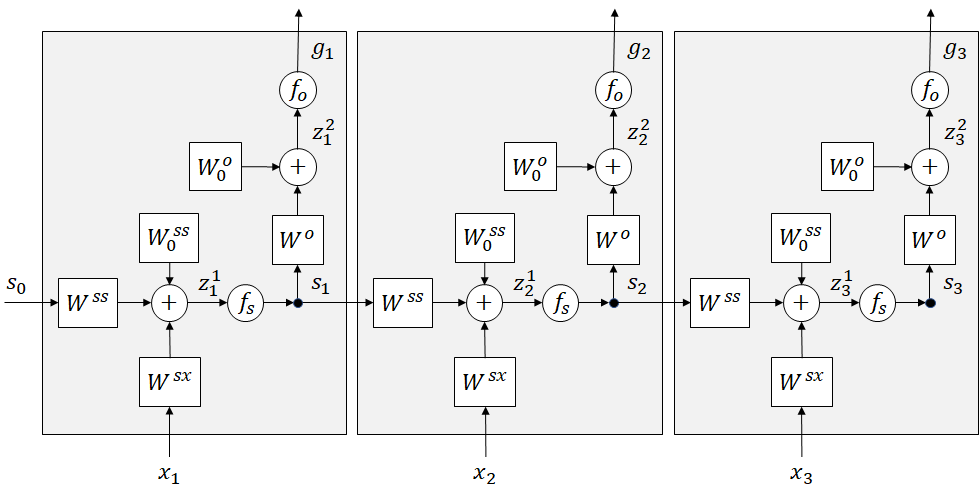
\includegraphics[width=\textwidth]{figures/rnn_unrolled_with_offsets.png}}

        Now,  we can see our problem as one of performing what is almost an
        ordinary back-propagation training procedure in a feed-forward neural
        network, but with the difference that the weight matrices are shared
        among the layers.  In many ways, this is similar to what ends up
        happening in a convolutional network, except in the conv-net, the
        weights are re-used spatially, and here, they are re-used temporally.
  \item
        Do the {\it forward pass}, to compute the predicted output sequence $g$:
        \begin{align}
          z_t^1 & = W^{sx}x_t + W^{ss}s_{t - 1} + W^{ss}_0 \\
          s_t   & = f_s(z_t^1)                             \\
          z_t^2 & = W^os_t + W_0^o                         \\
          g_t   & = f_o(z_t^2)
        \end{align}
  \item
        Do {\em backward pass} to compute the gradients. For both $W^{ss}$ and
        $W^{sx}$ we need to find
        \begin{align}
          \frac{d \mathcal{L}_\text{seq}(g,y)}{d W} & = \sum_{u = 1}^n\frac{d \mathcal{L}_\text{elt}(g_u, y_u)}{d W} ~~~~~~~~~~~~~~~~~~ \nonumber
        \end{align}
        Letting $\mathcal{L}_u = \mathcal{L}_\text{elt}(g_u, y_u)$ and using the {\em  total derivative}, which is a sum over all
        the ways in which $W$ affects $\mathcal{L}_u$, we have
        \begin{align}
          ~~~~ & = \sum_{u = 1}^n\sum_{t = 1}^n  \frac{\partial s_t}{\partial W} \frac{\partial \mathcal{L}_u}{\partial s_t}  \nonumber
        \end{align}
        Re-organizing, we have
        \begin{align}
          ~~~~ & = \sum_{t = 1}^n\frac{\partial s_t}{\partial W} \sum_{u =
            1}^n\frac{\partial \mathcal{L}_u}{\partial s_t} \nonumber
        \end{align}
        Because $s_t\ \text{only affects}\ \mathcal{L}_t, \mathcal{L}_{t + 1}, \dots, \mathcal{L}_n$,
        \begin{align}
          ~~~~~~~~~~~~~~~~~~~~ & = \sum_{t = 1}^n\frac{\partial s_t}{\partial W} \sum_{u = t}^n\frac{\partial \mathcal{L}_u}{\partial s_t} \nonumber \\
                               & = \sum_{t = 1}^n\frac{\partial s_t}{\partial W}
          \left(\frac{\partial \mathcal{L}_t}{\partial s_t} + \underbrace{\sum_{u = t +
              1}^n\frac{\partial \mathcal{L}_u}{\partial s_t}}_{\delta^{s_t}}\right) \; .\label{sumeq}
        \end{align}
        where $\delta^{s_t}$ is the dependence of the future loss (incurred after step $t$) on the
        state $S_t$.\note{That is, $\delta^{s_t}$ is how much we can
          blame state $s_t$ for all the future element losses.}

        We can compute this backwards, with $t$ going from $n$ down to $1$.
        The trickiest part is figuring out how early states contribute to later
        losses. We define the {\it{future loss}} after step $t$ to be
        \begin{equation}
          F_t = \sum_{u = t + 1}^{n}\mathcal{L}_\text{elt}(g_u, y_u) \;\;,
        \end{equation}
        so
        \begin{equation}
          \delta^{s_t} = \frac{\partial F_t}{\partial s_t}\;\;.
        \end{equation}
        At the last stage, $F_n = 0$ so $\delta^{s_n} = 0$.

        Now, working backwards,
        \begin{align}
          \delta^{s_{t -1}} & = \frac{\partial}{\partial s_{t - 1}}\sum_{u = t}^n\mathcal{L}_\text{elt}(g_u, y_u)                                                                                       \\
                            & = \frac{\partial s_t}{\partial s_{t - 1}} \frac{\partial}{\partial s_t}\sum_{u = t}^n\mathcal{L}_\text{elt}(g_u, y_u)                                                     \\
                            & = \frac{\partial s_t}{\partial s_{t - 1}} \frac{\partial}{\partial s_t}\left[\mathcal{L}_\text{elt}(g_t, y_t) + \sum_{u = t + 1}^n\mathcal{L}_\text{elt}(g_u, y_u)\right] \\
                            & = \frac{\partial s_t}{\partial s_{t - 1}} \left[\frac{\partial \mathcal{L}_\text{elt}(g_t, y_t)}{\partial s_t} + \delta^{s_t}\right]
        \end{align}
        Now, we can use the chain rule again to find the dependence of the
        element loss at time $t$ on the state  at that same time,
        \begin{equation}
          \underbrace{\frac{\partial \mathcal{L}_\text{elt}(g_t,
              y_t)}{\partial s_t}}_{(m \times 1)} = \underbrace{\frac{\partial
              z_t^2}{\partial s_t}}_{(m \times v)} ~
          \underbrace{\frac{\partial \mathcal{L}_\text{elt}(g_t, y_t)}{\partial
              z_t^2}}_{(v \times 1)}\;\;,
        \end{equation}
        and the dependence of the state at time $t$ on the state at the
        previous  time,
        %noting that we are performing an {\em elementwise}
        %multiplication between $W^T_{ss}$ and the vector of ${f^1}'$ values, $\partial
        %s_t /\partial z^1_t$:
        \iffalse
          \note{There  are two ways  to think about $\partial s_t  / \partial
              z_t$:  here, we take the view  that it is an $m \times 1$ vector and
            we multiply each column of $W^T$ by it.  Another, equally good,
            view, is that it is an $m \times m$ diagonal matrix, with the values
            along the diagonal, and then  this operation is a matrix multiply.
            Our software implementation will take the first view.
          }
        \fi
        \begin{equation}
          \underbrace{\frac{\partial s_t}{\partial s_{t - 1}}}_{(m \times m)}
          = \underbrace{\frac{\partial z_t^1}{\partial s_{t - 1}}}_{(m \times
            m)} \underbrace{\frac{\partial s_t}{\partial z_t^1}}_{(m
            \times m)} = {W^{ss}}^T \frac{\partial s_t}{\partial z_t^1}
        \end{equation} \\
        \begin{examplebox} Note that $\partial s_t /\partial z^1_t$
          is formally an $m \times m$ diagonal matrix, with the values
          along the diagonal being $f_{s}'(z_{t,i}^1)$, $1 \leq i \leq m$. But since this is a diagonal matrix, one could represent it as an $m \times 1$ vector $f_{s}'(z_t^1)$. In that case the product of the matrix ${W^{ss}}^T$ by the vector $f_{s}'(z_t^1)$, denoted ${W^{ss}}^T * f_{s}'(z_t^1)$, should be interpreted as follows: take the first column of the matrix ${W^{ss}}^T$ and multiply each of its elements by the first element of the vector $\partial s_t /\partial z^1_t$, then take the second column of the matrix ${W^{ss}}^T$ and multiply each of its elements by the second element of the vector $\partial s_t /\partial z^1_t$, and so on and so forth ...
        \end{examplebox}

        Putting this all together, we end up with
        \begin{equation}
          \delta^{s_{t - 1}} = \underbrace{{W^{ss}}^T \frac{\partial s_t}{\partial z_t^1}}_{\frac{\partial s_t}{\partial s_{t - 1}}} ~ \underbrace{\left({W^o}^T\frac{\partial{\mathcal{L}_t}}{\partial z_t^2} + \delta^{s_t}\right)}_{\frac{\partial F_{t - 1}}{\partial s_t}}
        \end{equation}

        We're almost there!  Now, we can describe the actual weight updates.
        Using Eq.~\ref{sumeq} and recalling the definition of
        $\delta^{s_t} = \partial F_t / \partial s_t$,
        as we iterate backwards, we can accumulate the terms in Eq.~\ref{sumeq}
        to get the gradient for the whole  loss.
        \iffalse
          \begin{align}
            \frac{ d \mathcal{L}_\text{seq}}{d W^{ss}} & +=
            \frac{\partial F_{t-1}}{\partial W^{ss}} =
            \frac{\partial z^1_t}{\partial W^{ss}} \frac{\partial s_t}{\partial z^1_t}
            \frac{\partial F_{t-1}}{\partial s_t}           \\
            \frac{ d \mathcal{L}_\text{seq}}{d W^{sx}} & +=
            \frac{\partial F_{t-1}}{\partial W^{sx}} =
            \frac{\partial z^1_t}{\partial W^{sx}} \frac{\partial s_t}{\partial z^1_t}
            \frac{\partial F_{t-1}}{\partial s_t}
          \end{align}
        \fi



        \begin{align}
          \frac{d \mathcal{L}_\text{seq}}{d W^{ss}} & = \sum_{t=1}^n
          \frac{d \mathcal{L}_\text{elt}(g_t, y_t)}{d W^{ss}} = \sum_{t=1}^n \frac{\partial z_t^1}{\partial W^{ss}} \frac{\partial s_t}{\partial z_t^1} \frac{\partial F_{t - 1}}{\partial s_t} \\
          \frac{d \mathcal{L}_\text{seq}}{d W^{sx}} & =  \sum_{t=1}^n
          \frac{d \mathcal{L}_\text{elt}(g_t, y_t)}{d W^{sx}} = \sum_{t=1}^n
          \frac{\partial z_t^1}{\partial W^{sx}} \frac{\partial s_t}{\partial z_t^1} \frac{\partial F_{t-1}}{\partial s_t}
        \end{align}
        We can handle $W^o$ separately;   it's easier because it does not
        affect future  losses  in the way that the other weight matrices do:
        \begin{equation}
          \frac{d\mathcal{L}_\text{seq}}{d W^o} = \sum_{t = 1}^n\frac{d \mathcal{L}_t}{d W^o} = \sum_{t = 1}^n\frac{\partial \mathcal{L}_t}{\partial
            z_t^2} \frac{\partial z_t^2}{\partial W^o}
        \end{equation}
        Assuming we have $\frac{\partial \mathcal{L}_t}{\partial z_t^2} = (g_t - y_t)$,
        (which ends up being true for squared loss, softmax-NLL, etc.), then
        \begin{equation}
          \underbrace{\frac{d \mathcal{L}_\text{seq}}{d W^o}}_{v \times m} = \sum_{t=1}^n \underbrace{(g_t - y_t)}_{v \times 1} ~ \underbrace{s_t^T}_{1 \times m} \; .
        \end{equation}

        Whew!
\end{enumerate}
\question{Derive the updates for the offsets $W^{ss}_0$ and $W^o_0$.}

%%%%%%%%%%%%%%%%%%%%%%%%%%%%%%%%%%%%%%%%%%%%%%%%%%%%%%%%%%%%%%%%%%%%%%%%%%%%%
\section{Vanishing gradients and gating mechanisms}
\label{lstm}
\label{sec-rnn_lstm}

Let's take a careful look at the backward propagation of the gradient
along the sequence:
\begin{equation}
  \delta^{s_{t -1}} = \frac{\partial s_t}{\partial s_{t - 1}} ~
  \left[\frac{\partial \mathcal{L}_\text{elt}(g_t, y_t)}{\partial s_t}
    + \delta^{s_t}\right]\;\;.
\end{equation}
Consider a case where only the output at the end of the sequence is
incorrect, but it depends critically, via the weights,  on the input
at time 1.   In this case, we will multiply the loss at step $n$ by
\begin{equation}
  \frac{\partial s_2}{\partial s_1} \frac{\partial s_3}{\partial
    s_2} \cdots \frac{\partial s_n}{\partial s_{n-1}}\;\;.
\end{equation}
In general, this quantity will either grow or shrink exponentially
with the length of the sequence, and make it very difficult to train.
\question{The last time we talked about exploding and vanishing
  gradients, it was to justify per-weight adaptive step sizes.  Why is
  that not a solution to the problem this time?}

An important insight that really made recurrent networks work well on
long sequences is the idea of {\em gating}\index{recurrent neural network!gating}.

\subsection{Simple gated recurrent networks}

A computer only ever updates some parts of its memory on each
computation cycle.  We can take this idea and use it to make our
networks more able to retain state values over time and to make the
gradients better-behaved.  We will add a new component to our network,
called a {\em gating network}\index{gating network}.  Let $g_t$ be a $m \times 1$ vector of
values and let $W^{gx}$ and $W^{gs}$ be $m \times l$ and $m \times m$
weight matrices, respectively.  We will compute $g_t$ as
\note{It can have an offset, too, but we are omitting it for simplicity.}
\begin{equation}
  g_t = \text{sigmoid}(W^{gx} x_t + W^{gs} s_{t-1})
\end{equation}
and then change the computation of $s_t$ to be
\begin{equation}
  s_t = (1 - g_t) *  s_{t-1} + g_t * f_s(W^{sx}x_t + W^{ss}
  s_{t-1} + W^{ss}_0)\;\;,
\end{equation}
where $*$ is component-wise multiplication.  We can see, here, that
the output of the gating network is deciding, for each dimension of
the state, how much it should be updated now.  This mechanism makes it
much easier for the network to learn to,  for example, ``store'' some
information in some dimension of the state, and then not change it
during future state updates, or change it only under certain
conditions on the input or other aspects of the state.
\question{Why is it important that the activation function for $g$ be
  a sigmoid?}

\subsection{Long short-term memory}

The idea of gating networks can be applied to make a state machine
that is even more like a computer memory, resulting in a type of
network called an {\sc  lstm}\index{long short-term memory} for ``long short-term memory.''
\note{Yet another awesome name for a neural network!}  We won't go
into the details here,  but the basic idea is that there is a memory
cell (really, our state vector) and three (!) gating networks.  The
  {\em input} gate selects (using a ``soft''  selection as in the gated
network above) which dimensions of the state will be updated  with new
values;  the {\em forget} gate decides which dimensions of the state
will have its old values  moved toward 0, and the {\em  output} gate
decides which dimensions of the state will be used to compute the
output value.  These networks have been used in applications like
language translation with really amazing results.  A diagram of the
architecture is shown below:
\begin{center}
  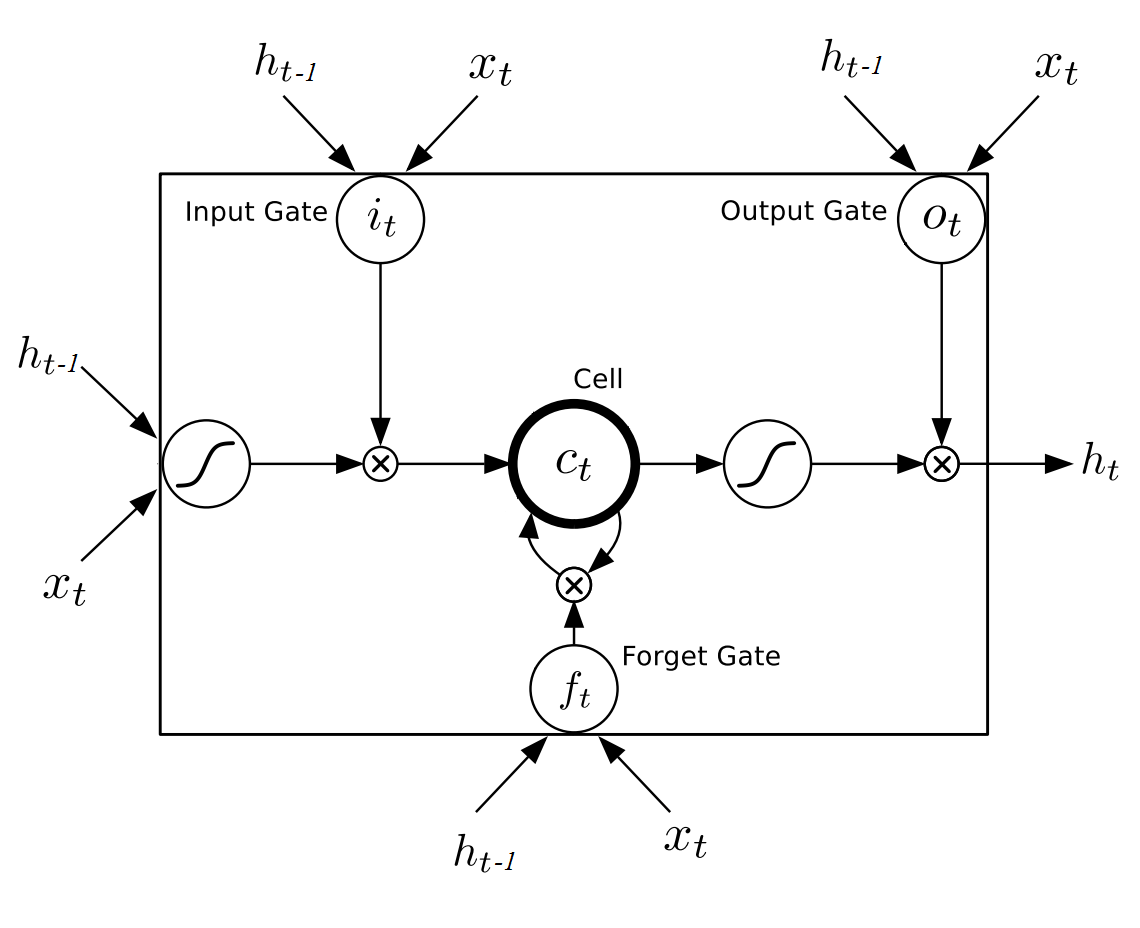
\includegraphics[scale = 0.7]{figures/lstm.png}
\end{center}


%%% Local Variables:
%%% mode: latex
%%% TeX-master: "top"
%%% End:

